\documentclass[aspectratio=169]{beamer}
\usetheme{metropolis}

\usepackage[T1]{fontenc}
\usepackage{booktabs}
\usepackage{graphicx}
\usepackage{tabularx}
\usepackage{tikz}
\usetikzlibrary{arrows.meta,positioning,shapes.geometric}

\metroset{
  progressbar=frametitle,
  numbering=fraction,
  block=fill
}

\definecolor{ILABNavy}{HTML}{213547}
\definecolor{ILABTeal}{HTML}{0F766E}
\definecolor{ILABAmber}{HTML}{B7791F}
\definecolor{ILABSlate}{HTML}{475569}
\definecolor{ILABRed}{HTML}{B91C1C}
\setbeamercolor{normal text}{fg=ILABNavy,bg=white}
\setbeamercolor{frametitle}{fg=white,bg=ILABNavy}
\setbeamercolor{progress bar}{fg=ILABTeal,bg=ILABSlate!20}
\setbeamercolor{alerted text}{fg=ILABRed}
\setbeamercolor{block title}{fg=white,bg=ILABTeal}
\setbeamercolor{block body}{fg=ILABNavy,bg=ILABTeal!8}

\newcommand{\pathref}[1]{{\scriptsize\texttt{#1}}}
\newcommand{\tightsep}{\vspace{0.35em}}
\newcommand{\yes}{\textcolor{ILABTeal}{ready}}
\newcommand{\warn}{\textcolor{ILABAmber}{operator-gated}}
\newcommand{\risk}{\textcolor{ILABRed}{risk}}

\title{Smart i-LAB Testbed}
\subtitle{Technical Review: IoT platform, Digital Twin, CV occupancy, and operations}
\author{pctiope/smart-i-lab-testbed}
\institute{}
\date{May 2026}

\begin{document}

\begin{frame}[plain]
\vfill
{\usebeamerfont{title}\color{ILABNavy}\LARGE Smart i-LAB Testbed\par}
\vspace{0.8em}
{\usebeamerfont{subtitle}\color{ILABSlate}Technical Review: IoT platform, Digital Twin, CV occupancy, and operations\par}
\vspace{1.6em}
{\usebeamerfont{author}\color{ILABNavy}pctiope/smart-i-lab-testbed\par}
\vspace{0.4em}
{\usebeamerfont{date}\color{ILABSlate}May 2026\par}
\vfill
\end{frame}

\begin{frame}{Review Objective}
\begin{columns}[T,onlytextwidth]
\column{0.52\textwidth}
\begin{block}{What this deck documents}
\begin{itemize}
  \item The current combined repository after the Zone 5 mmWave recency update landed on \texttt{main}.
  \item The end-to-end data path from lab devices to TimescaleDB, REST, Digital Twin, and CV/ML consumers.
  \item Operational boundaries between source deploy, staging Compose, production systemd, retraining, and model delivery.
\end{itemize}
\end{block}
\column{0.42\textwidth}
\begin{block}{What is intentionally excluded}
\begin{itemize}
  \item API keys, populated \texttt{.env} values, RTSP secrets, MQTT passwords, and private tokens.
  \item Generated runtime state under \texttt{data/}, \texttt{model/runs/}, and \texttt{logs/}.
\end{itemize}
\end{block}
\end{columns}
\end{frame}

\begin{frame}{System Purpose}
\begin{columns}[T,onlytextwidth]
\column{0.48\textwidth}
\textbf{Lab platform}
\begin{itemize}
  \item Smart i-LAB Room 308 testbed for sensor acquisition, device control, and remote experimentation.
  \item MQTT devices and Home Assistant inputs are normalized into TimescaleDB-backed history.
  \item REST endpoints provide read paths for Digital Twin and model consumers, plus controlled actuator paths.
\end{itemize}
\column{0.48\textwidth}
\textbf{Occupancy intelligence}
\begin{itemize}
  \item Zone 5 package trains a dedicated CNN-1D occupancy model using CV labels plus AIR-1, power, mmWave, SEN55, and time features.
  \item AIR1 all-zones package trains one shared model over zones 1--15 using two-camera per-zone labels.
  \item Live dashboards expose model outputs, CV ground truth, health, and video streams.
\end{itemize}
\end{columns}
\end{frame}

\begin{frame}[shrink=6]{Repository Map}
\scriptsize
\begin{tabularx}{\textwidth}{@{}lX@{}}
\toprule
\textbf{Path} & \textbf{Role} \\
\midrule
\pathref{SSL-IoT1-REST/} & Express REST API, OpenAPI files, Dockerfile, auth, device reads, actuator endpoints. \\
\pathref{Smart-iLAB-Python-Files/} & ESP, Zigbee, and Sensibo databridges from MQTT or Home Assistant into TimescaleDB. \\
\pathref{Smart-iLab\_DigitalTwin/} & Vite and Three.js Digital Twin, built and served by nginx in Docker. \\
\pathref{migrations/} & Versioned schema migrations for core tables, registries, hypertables, and retrofit steps. \\
\pathref{zone5\_cv\_time\_features\_package/} & Zone 5 CV labels, sensor joins, training, promotion, live inference, dashboard, and CI/CD docs. \\
\pathref{air1\_all\_zones\_cv\_time\_features\_package/} & Shared all-zones AIR1 model, two-camera labels, collector, trainer, and operations app. \\
\pathref{docs/}, \pathref{.github/workflows/} & IoT1 audit/remediation docs and production/staging workflow automation. \\
\bottomrule
\end{tabularx}
\end{frame}

\begin{frame}{End-To-End Architecture}
\centering
\resizebox{0.98\textwidth}{!}{%
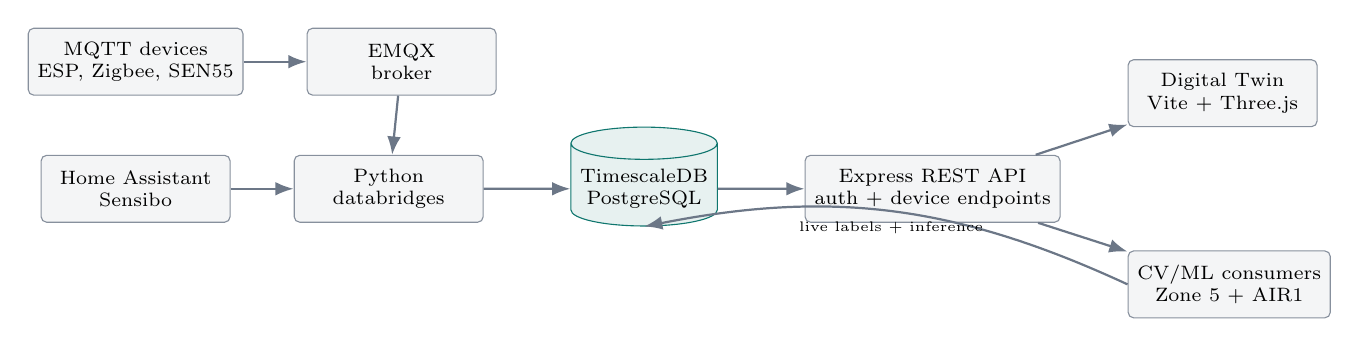
\begin{tikzpicture}[
  node distance=0.75cm and 0.8cm,
  box/.style={draw=ILABSlate!65, rounded corners=2pt, fill=ILABSlate!6, align=center, minimum width=2.4cm, minimum height=0.85cm, font=\scriptsize},
  store/.style={draw=ILABTeal, cylinder, shape border rotate=90, aspect=0.22, fill=ILABTeal!10, align=center, minimum height=1.0cm, font=\scriptsize},
  flow/.style={-Latex, thick, draw=ILABSlate!80}
]
\node[box] (devices) {MQTT devices\\ESP, Zigbee, SEN55};
\node[box, below=of devices] (ha) {Home Assistant\\Sensibo};
\node[box, right=of devices] (emqx) {EMQX\\broker};
\node[box, right=of ha] (bridges) {Python\\databridges};
\node[store, right=1.1cm of bridges] (db) {TimescaleDB\\PostgreSQL};
\node[box, right=1.1cm of db] (rest) {Express REST API\\auth + device endpoints};
\node[box, above right=0.35cm and 0.85cm of rest] (dt) {Digital Twin\\Vite + Three.js};
\node[box, below right=0.35cm and 0.85cm of rest] (cv) {CV/ML consumers\\Zone 5 + AIR1};

\draw[flow] (devices) -- (emqx);
\draw[flow] (emqx) -- (bridges);
\draw[flow] (ha) -- (bridges);
\draw[flow] (bridges) -- (db);
\draw[flow] (db) -- (rest);
\draw[flow] (rest) -- (dt);
\draw[flow] (rest) -- (cv);
\draw[flow] (cv.west) to[bend right=18] node[below,font=\tiny] {live labels + inference} (db.south);
\end{tikzpicture}
}
\end{frame}

\begin{frame}{Data And Migration Model}
\begin{columns}[T,onlytextwidth]
\column{0.5\textwidth}
\textbf{Schema-as-code}
\begin{itemize}
  \item \pathref{migrations/apply.py} applies lexical SQL migrations once and records versions in \texttt{schema\_migrations}.
  \item Core tables cover users, transactions, groups, error logs, and device registries.
  \item Per-device sensor tables are discovered lazily by databridges.
\end{itemize}
\column{0.46\textwidth}
\textbf{TimescaleDB shape}
\begin{itemize}
  \item Device tables are converted to hypertables when created or retrofitted.
  \item The current retrofit adds \texttt{PRIMARY KEY(timestamp)} where duplicate timestamps do not block it.
  \item Dirty legacy tables remain an operator cleanup item, with dedupe tooling documented.
\end{itemize}
\end{columns}
\end{frame}

\begin{frame}{REST API And Security Status}
\small
\begin{tabularx}{\textwidth}{@{}lXX@{}}
\toprule
\textbf{Area} & \textbf{Current state} & \textbf{Review note} \\
\midrule
Auth & API-key checks, access-level validation, query cache. & CV packages send \texttt{x-api-key}; Bearer headers are ignored harmlessly. \\
SQL safety & User, group, transaction, and ingest paths parameterized or allow-listed. & The historical audit lists 46 findings closed at code level. \\
Runtime hardening & Helmet, rate limits on auth/write paths, request timeout, body cap, non-root containers. & Behavioral QA still depends on lab infrastructure. \\
Compatibility & AIR1 and Zone 5 consumer endpoint shapes are unchanged. & Recommended client timeout remains below server cap. \\
\bottomrule
\end{tabularx}
\tightsep
\pathref{docs/IOT1\_AUDIT.md}, \pathref{docs/IOT1\_REMEDIATION.md}, and \pathref{docs/IOT1\_CV\_COMPATIBILITY.md} capture the evidence trail.
\end{frame}

\begin{frame}{Digital Twin Frontend}
\begin{columns}[T,onlytextwidth]
\column{0.48\textwidth}
\textbf{Role}
\begin{itemize}
  \item Web visualization of lab status and selected controls.
  \item Demonstrates the REST API as the integration surface for users and downstream tools.
  \item Built with Vite and bundled Three.js assets.
\end{itemize}
\column{0.48\textwidth}
\textbf{Current packaging}
\begin{itemize}
  \item Multi-stage Docker build: Node builds static assets, nginx serves them.
  \item API base URL comes from build-time \texttt{VITE\_API\_URL}.
  \item Content-Security-Policy is present but deliberately permissive pending later tightening.
\end{itemize}
\end{columns}
\end{frame}

\begin{frame}{CV/ML Package Split}
\small
\begin{tabularx}{\textwidth}{@{}lXX@{}}
\toprule
\textbf{Dimension} & \textbf{Zone 5} & \textbf{AIR1 all-zones} \\
\midrule
Model scope & One model for Zone 5. & One shared model over zones 1--15. \\
Rows & One row per 10-second timestamp. & One row per timestamp and \texttt{zone\_id}. \\
Labels & YOLO person count aggregated into \texttt{zone\_occupied}. & Two-camera mask labels aggregated into \texttt{occupied}. \\
Inputs & AIR-1, smart plug, mmWave, SEN55, time features. & AIR-1, shared SEN55, missing indicators, time features. \\
Excluded & Missingness is diagnostic, not a model input. & Power and mmWave are outside the contract. \\
Serving & Zone 5 dashboard, SSE, history, MJPEG. & All-zones ops view, two MJPEG feeds, per-zone probabilities. \\
\bottomrule
\end{tabularx}
\end{frame}

\begin{frame}{Zone 5 Occupancy Pipeline}
\centering
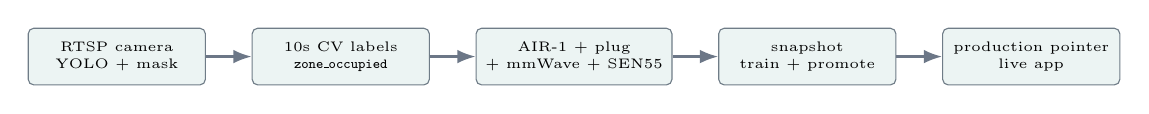
\begin{tikzpicture}[
  node distance=0.58cm,
  flowstep/.style={draw=ILABNavy!65, fill=ILABTeal!8, rounded corners=2pt, align=center, minimum width=2.25cm, minimum height=0.72cm, font=\tiny},
  flow/.style={-Latex, thick, draw=ILABSlate!80}
]
\node[flowstep] (cam) {RTSP camera\\YOLO + mask};
\node[flowstep, right=of cam] (cv) {10s CV labels\\\texttt{zone\_occupied}};
\node[flowstep, right=of cv] (join) {AIR-1 + plug\\+ mmWave + SEN55};
\node[flowstep, right=of join] (train) {snapshot\\train + promote};
\node[flowstep, right=of train] (serve) {production pointer\\live app};
\draw[flow] (cam) -- (cv);
\draw[flow] (cv) -- (join);
\draw[flow] (join) -- (train);
\draw[flow] (train) -- (serve);
\end{tikzpicture}
\tightsep
\begin{itemize}
  \item Persistent services: person counter, MQTT aggregator, SEN55 collector, live collector, live app, Vite frontend.
  \item Trainer timer is separate from collection and uses a retrain lock plus immutable snapshots.
  \item Promotion atomically updates \texttt{model/production\_run.txt}; the live app reloads on pointer change.
\end{itemize}
\end{frame}

\begin{frame}[shrink=4]{Zone 5 Feature Contract}
\small
\begin{columns}[T,onlytextwidth]
\column{0.5\textwidth}
\textbf{Raw signals retained}
\begin{itemize}
  \item AIR-1: temperature, RH, CO2, PM2.5.
  \item Smart plug: \texttt{power\_s5}.
  \item mmWave: \texttt{mmwave\_s5}.
  \item SEN55: PM, temperature, humidity, VOC, NOx.
  \item Time: hour and day-of-week sin/cos.
\end{itemize}
\column{0.46\textwidth}
\textbf{Current contract}
\begin{itemize}
  \item Contract marker: \texttt{zone5\_mmwave\_recency\_v1}.
  \item Added past-only mmWave recency features:
    \texttt{1m}, \texttt{3m}, \texttt{5m} occupied fractions and minutes since last occupied.
  \item Missing indicators remain metadata/diagnostics and are excluded from model inputs.
  \item Legacy missingness-decoupled artifacts are supported for live loading, but new training writes the recency contract.
\end{itemize}
\end{columns}
\end{frame}

\begin{frame}{Zone 5 Live Dashboard}
\small
\begin{columns}[T,onlytextwidth]
\column{0.5\textwidth}
\textbf{Backend API}
\begin{itemize}
  \item \texttt{/api/health}: model, collector, RTSP, and freshness state.
  \item \texttt{/api/current}: latest inference and sensor context.
  \item \texttt{/api/history}: prediction history, CV labels, mmWave lookback context.
  \item \texttt{/api/video.mjpg}: file-backed annotated frame stream.
\end{itemize}
\column{0.46\textwidth}
\textbf{Frontend behavior}
\begin{itemize}
  \item Vite dashboard displays probability, CV truth, history, MSE, sensor sparklines, and split-pane video.
  \item New history view surfaces mmWave lookback fraction rather than only the instantaneous bit.
  \item Generated data, model runs, logs, and runtime environment values remain out of git.
\end{itemize}
\end{columns}
\end{frame}

\begin{frame}{AIR1 All-Zones Pipeline}
\centering
\resizebox{0.98\textwidth}{!}{%
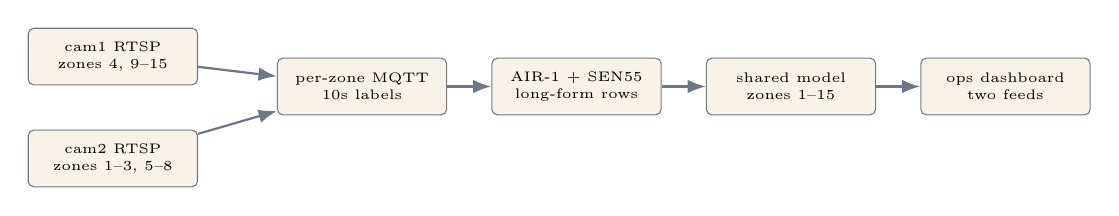
\begin{tikzpicture}[
  node distance=0.56cm,
  flowstep/.style={draw=ILABNavy!65, fill=ILABAmber!10, rounded corners=2pt, align=center, minimum width=2.15cm, minimum height=0.72cm, font=\tiny},
  flow/.style={-Latex, thick, draw=ILABSlate!80}
]
\node[flowstep] (cam1) {cam1 RTSP\\zones 4, 9--15};
\node[flowstep, below=of cam1] (cam2) {cam2 RTSP\\zones 1--3, 5--8};
\node[flowstep, right=1.0cm of cam1, yshift=-0.38cm] (labels) {per-zone MQTT\\10s labels};
\node[flowstep, right=of labels] (join) {AIR-1 + SEN55\\long-form rows};
\node[flowstep, right=of join] (model) {shared model\\zones 1--15};
\node[flowstep, right=of model] (app) {ops dashboard\\two feeds};
\draw[flow] (cam1) -- (labels);
\draw[flow] (cam2) -- (labels);
\draw[flow] (labels) -- (join);
\draw[flow] (join) -- (model);
\draw[flow] (model) -- (app);
\end{tikzpicture}
}
\tightsep
\begin{itemize}
  \item Labels are keyed by \texttt{timestamp + zone\_id}; missing camera coverage stays null, not false zero.
  \item \texttt{zone\_id} is retained for grouping, windows, audit, splits, and display, but is not a model input.
  \item Production inference is gated by \texttt{model/production\_run.txt}.
\end{itemize}
\end{frame}

\begin{frame}[shrink=6]{Deployment Surfaces}
\scriptsize
\begin{tabularx}{\textwidth}{@{}lXX@{}}
\toprule
\textbf{Surface} & \textbf{Purpose} & \textbf{Boundary} \\
\midrule
Root Compose & IoT1 REST API, Digital Twin, databridges. & External production PG/EMQX/HA by default; dev overlay can colocate PG and EMQX. \\
Zone 5 systemd & Production source deployment for live services. & User-systemd services, production ports \texttt{8000}/\texttt{8015}; source deploy does not start trainer. \\
Zone 5 Compose & Staging deployment path. & Separate branch/path and staging ports \texttt{8005}/\texttt{8016}. \\
Model delivery & Promotion of generated model artifacts. & Separate from source deploy; protects generated state and production pointers. \\
AIR1 systemd/Compose & Parallel package deployment surfaces. & Same collection/training split, no mmWave or power contract import. \\
\bottomrule
\end{tabularx}
\end{frame}

\begin{frame}{Testing And Verification}
\begin{columns}[T,onlytextwidth]
\column{0.48\textwidth}
\textbf{Code validation}
\begin{itemize}
  \item Python compile checks for Zone 5 modules and web app.
  \item CV ground-truth unit coverage for contracts, splits, promotion gates, parser behavior, live loader checks, and UI affordances.
  \item Docker Compose config/build checks in CI/CD paths.
\end{itemize}
\column{0.48\textwidth}
\textbf{Operations validation}
\begin{itemize}
  \item Health endpoints for live apps and Vite frontend.
  \item Production pointers: \texttt{current\_run.txt}, \texttt{production\_run.txt}, and retrain status.
  \item Trainer locks avoid overlapping expensive fits.
  \item IoT1 migration and smoke-test sequence remains operator-gated.
\end{itemize}
\end{columns}
\end{frame}

\begin{frame}[shrink=6]{Current Status Snapshot}
\scriptsize
\begin{tabularx}{\textwidth}{@{}lXl@{}}
\toprule
\textbf{Area} & \textbf{Status} & \textbf{Marker} \\
\midrule
IoT1 code remediation & Audit findings closed at code level; deployment cutover pending backup, migration, deploy, smoke test, and log tailing. & \warn \\
Zone 5 source & mmWave recency contract is now on \texttt{main}; package tests and compile checks pass locally. & \yes \\
Zone 5 operations & Production systemd and staging Compose are intentionally separate. Retraining/model delivery remain distinct workflows. & \yes \\
AIR1 all-zones & Shared-model package has persistent service/timer surfaces and preserved null labels for missing camera coverage. & \yes \\
Generated artifacts & Runtime data, logs, model runs, and populated env files stay out of source control. & \yes \\
\bottomrule
\end{tabularx}
\end{frame}

\begin{frame}[shrink=4]{Risks To Track}
\small
\begin{columns}[T,onlytextwidth]
\column{0.5\textwidth}
\textbf{Platform risks}
\begin{itemize}
  \item Live IoT1 database migration still requires backup and operator execution.
  \item Legacy per-device tables with duplicate timestamps need dedupe before every table can receive the timestamp primary key.
  \item Full behavioral QA requires lab LAN, TimescaleDB, EMQX, Home Assistant, and devices.
\end{itemize}
\column{0.46\textwidth}
\textbf{Model and runtime risks}
\begin{itemize}
  \item Training quality depends on enough both-class CV label coverage across calendar windows.
  \item Upstream AIR-1 outages can degrade live feature freshness.
  \item New contract versions require careful artifact compatibility and dashboard context updates.
\end{itemize}
\end{columns}
\end{frame}

\begin{frame}{Roadmap}
\begin{enumerate}
  \item Complete IoT1 production cutover: backup, migrations, hardened container deploy, admin-key smoke test, and subscriber log watch.
  \item Finish table cleanup for duplicate timestamp histories, then re-run the hypertable/primary-key retrofit.
  \item Keep Zone 5 manual-first retraining proof before enabling scheduled production retraining.
  \item Add monitoring around model freshness, label class balance, promotion outcomes, and upstream API latency.
  \item Maintain AIR1 and Zone 5 contract separation: AIR1 stays AIR-1/SEN55/time only; Zone 5 owns power and mmWave.
\end{enumerate}
\end{frame}

\begin{frame}{Review Takeaways}
\begin{itemize}
  \item The repository is a combined lab platform plus two CV/ML occupancy packages; the integration point is the hardened IoT1 REST API over TimescaleDB-backed history.
  \item Zone 5 now represents mmWave as both an instantaneous signal and past-only recency features, while keeping missingness out of the model input contract.
  \item Deployment is intentionally split: IoT1 cutover is operator-gated, Zone 5 production stays user-systemd, Compose is staging, and model promotion is separate from source deploy.
  \item The remaining work is operational discipline: cutover, cleanup, monitoring, and controlled retraining automation.
\end{itemize}
\end{frame}

\begin{frame}{Source Anchors}
\small
\begin{tabularx}{\textwidth}{@{}lX@{}}
\toprule
\textbf{Topic} & \textbf{Primary source paths} \\
\midrule
IoT1 architecture and remediation & \pathref{README.md}, \pathref{docs/STATUS.md}, \pathref{docs/IOT1\_REMEDIATION.md} \\
Migrations and schema model & \pathref{migrations/README.md}, \pathref{migrations/*.sql} \\
Zone 5 pipeline and contract & \pathref{zone5\_cv\_time\_features\_package/PIPELINE.md}, \pathref{zone5/feature\_contract.py} \\
AIR1 all-zones contract & \pathref{air1\_all\_zones\_cv\_time\_features\_package/PIPELINE.md}, \pathref{README.md} \\
Deployment and CI/CD & \pathref{zone5\_cv\_time\_features\_package/CICD\_SYSTEMD.md}, \pathref{CICD\_DOCKER\_COMPOSE.md}, \pathref{.github/workflows/} \\
\bottomrule
\end{tabularx}
\end{frame}

\end{document}
